% !TEX program = xelatex
\documentclass{iopjournal}

% ── 宏包（iopjournal.cls 已加载 graphicx, xcolor, hyperref）──
\usepackage{amsmath,amssymb}
\usepackage{booktabs}
\usepackage{multirow}
\usepackage{algorithm}
\usepackage{algpseudocode}
\usepackage{siunitx}
\usepackage[caption=false]{subfig}
\usepackage{xeCJK}

% ── CJK 字体 ──────────────────────────────────────────────────
\setCJKmainfont{Noto Serif CJK SC}
\setCJKsansfont{Noto Sans CJK SC}
\setCJKmonofont{Noto Sans CJK SC}

\graphicspath{{figs/}}
\sisetup{round-mode=places, round-precision=3}

% ── 自定义命令 ─────────────────────────────────────────────────
\newcommand{\ie}{\textit{i.e.}}
\newcommand{\eg}{\textit{e.g.}}
\newcommand{\etal}{\textit{et al.}}

\begin{document}

\articletype{Paper}

% ══════════════════════════════════════════════════════════════
\title{CNN-PDDQN：一种改进的面向森林场景的UGV深度强化学习运动规划方法}

\author{Firstname Lastname$^1$, Firstname Lastname$^2$ and Firstname Lastname$^{2,*}$}

\affil{$^1$Affiliation 1}

\affil{$^2$Affiliation 2}

\affil{$^*$Author to whom any correspondence should be addressed.}

\email{e-mail@e-mail.com}

\keywords{可通行性评估, 阿克曼UGV, 深度强化学习, 运动规划, CNN-PDDQN}

% ══════════════════════════════════════════════════════════════
\begin{abstract}
森林巡检与作业要求自主地面无人车（UGV）在树干密集、地形起伏的非结构化环境中，实时生成满足运动学约束的安全可执行轨迹。针对传统图搜索与采样规划在狭窄通道中计算开销大、轨迹可控性不足的问题，提出一种面向森林场景的深度强化学习运动规划方法。首先利用FAST-LIO2构建先验三维点云地图，并基于可通行性评估生成二维占据栅格及到目标的代价场；随后将规划过程建模为马尔可夫决策过程，设计基于CNN-PDDQN的策略学习框架，并结合双圆足迹碰撞近似与进度/平滑约束构造奖励函数。推理阶段引入在线动作掩码与短视滚动预测的可行域过滤，剔除必碰撞或低收益动作，并配合回退机制与分层验证以降低无效动作选择与振荡风险。随机森林仿真与真实林地实验表明，该方法在路径质量与规划效率之间取得更优折中：仿真长路径任务中CNN-PDDQN生成最短路径$40.197$\,m且规划耗时仅$0.269$\,s，真实林地长路径中MLP-DDQN成功率达$95\%$、规划耗时仅$0.134$\,s，均显著低于传统算法。消融实验进一步验证了奖励函数设计与纯DQN直接控制策略的有效性。
\end{abstract}

% keywords already declared above via \keywords{}

% ══════════════════════════════════════════════════════════════
\section{介绍}\label{sec:intro}

近年来，随着林地巡检、生态监测及林下资源作业等任务需求的增加，地面无人车（UGV）在森林等非结构化环境中的自主通行能力面临着严峻挑战。与城市道路等具备清晰几何特征的结构化场景显著不同，林间环境通常具有地表起伏剧烈、障碍物（如树干）分布密集且无规则等特点。在这一复杂条件下，路径规划算法面临着双重压力：一方面需要在障碍物稠密的区域生成严格无碰撞的安全轨迹，另一方面需在极有限的狭窄间隙中实现灵活穿梭。

现有的运动规划算法大致可分为三类：（1）传统算法；（2）优化算法；（3）基于强化学习的算法。

\subsection{传统规划方法}

传统规划方法在工程上应用广泛，包括基于图的方法和基于采样的方法等。传统方法优点是原理成熟，缺点是路径易不连续、易陷局部最优、计算效率有限。

其中，基于图搜索的方法中，Hybrid\,A*由于能够在搜索扩展过程中同步完成碰撞检测、并严格满足车辆运动学约束而被广泛采用。Jiang~\etal~\cite{jiang2025hybrid}面向果园窄通道贴行导航，构建了``改进D*~Lite全局规划+窄段Hybrid\,A*局部重规划+轨迹平滑''的混合框架。Lian~\etal~\cite{lian2023trajectory}针对狭窄环境代客泊车，先以增强Hybrid\,A*生成高质量初值，再引入非线性最优控制进行二次优化。Pang~\etal~\cite{pang2022curvature}在自动泊车场景中提出基于Hybrid\,A*的反向搜索与碰撞剪枝策略。Thoresen~\etal~\cite{thoresen2021path}将地形可通行性评估融入Hybrid\,A*代价函数，使UGV更倾向于选择风险更低、可通过性更强的路径。Zhang~\etal~\cite{zhang2024twostage}面向露天矿大尺度场景提出两阶段二分Hybrid\,A*。总体而言，图搜索算法能够较高效地给出可行路线，但在长路径下引入碰撞检测往往会显著增加计算开销。

基于采样的规划方法通常以PRM、RRT及其改进RRT*为代表。Jian~\etal~\cite{jian2024path}提出PE-RRT*，将支撑平面估计与RRT*的采样/扩展过程紧密耦合。Jiang~\etal~\cite{jiang2022r2rrt}提出R2-RRT*，在RRT*搜索过程中显式引入不确定地形条件下的可靠性指标。Tian~\etal~\cite{tian2023driving}提出PF-RRT*，通过势场对障碍物与越野风险进行连续表征。Yin~\etal~\cite{yin2023efficient}在RRT*框架中耦合替代模型以近似可靠性评估。

\subsection{基于优化的算法}

基于优化的算法主要包括遗传算法（GA）、蚁群优化算法（ACO）、粒子群算法（PSO）以及人工蜂群算法（ABC）等。Cai~\etal~\cite{cai2024cooperative}提出基于优化ACO的合作路径规划方法。Huo~\etal~\cite{huo2024smooth}提出改进ACO结合B样条曲线的平滑规划思路。Li~\etal~\cite{li2023mixing}将ACO与ABC进行混合设计。Xu~\etal~\cite{xu2022quartic}引入四次Bezier过渡曲线并结合改进PSO。Yildirim和Akay~\cite{yildirim2025efficient}在栅格地图框架下设计改进ABC算法。

\subsection{基于强化学习的方法}

基于强化学习（RL）的路径规划方法通常以DQN等深度强化学习为代表。Kumar~\etal~\cite{kumar2025dsqn}提出DSQN，将脉冲神经元机制引入深度Q学习框架。Li和Wang~\cite{li2025iqaco}将Q评估机制显式融入ACO，提出改进的IQACO。Maoudj和Hentout~\cite{maoudj2020optimal}基于Q-learning构建最优路径规划框架。Sichkar~\cite{sichkar2019reinforcement}对Q-learning与SARSA等强化学习算法进行对比分析。Xu~\etal~\cite{xu2026rl}提出强化学习驱动的启发式路径规划思路。Zhou~\etal~\cite{zhou2018dqn}设计基于DQN的移动机器人路径规划方法。然而，将RL直接应用于森林狭窄通道规划仍存在突出困难：阿克曼车辆的非完整约束导致大量动作不可行；非结构化环境中可通行区域提取容易受地表起伏、落叶堆积、点云稀疏及噪声影响。

\subsection{本文贡献}

针对上述问题，本文提出一套面向森林非结构化狭窄障碍场景的UGV运动规划框架，主要贡献如下：

\begin{enumerate}
  \item 提出一套``先验点云建图---可通行性分割---二维占据栅格/代价场构建---运动规划''的完整流程，提高可通行区域提取与规划输入的可靠性。
  \item 提出基于CNN-PDDQN的UGV运动规划策略，结合两圆足迹与代价场设计，将安全裕度、进度与可控性约束统一纳入MDP建模与奖励函数中。
  \item 提出面向狭窄障碍场景的在线动作掩码与可行域过滤机制，通过短视预测筛除低收益动作，提升规划稳定性与实时性。
  \item 在多场景仿真与真实林地实验中验证了方法的有效性。
\end{enumerate}

% ══════════════════════════════════════════════════════════════
\section{方法}\label{sec:method}

如图~\ref{fig:framework}所示，本文提出一种面向森林场景的UGV运动规划框架：首先基于FAST-LIO2构建先验点云地图；随后通过可通行性评估实现点云分割，并生成二维栅格地图；最后在此基础上设计CNN-PDDQN深度强化学习路径规划算法。

\begin{figure}[t]
\centering
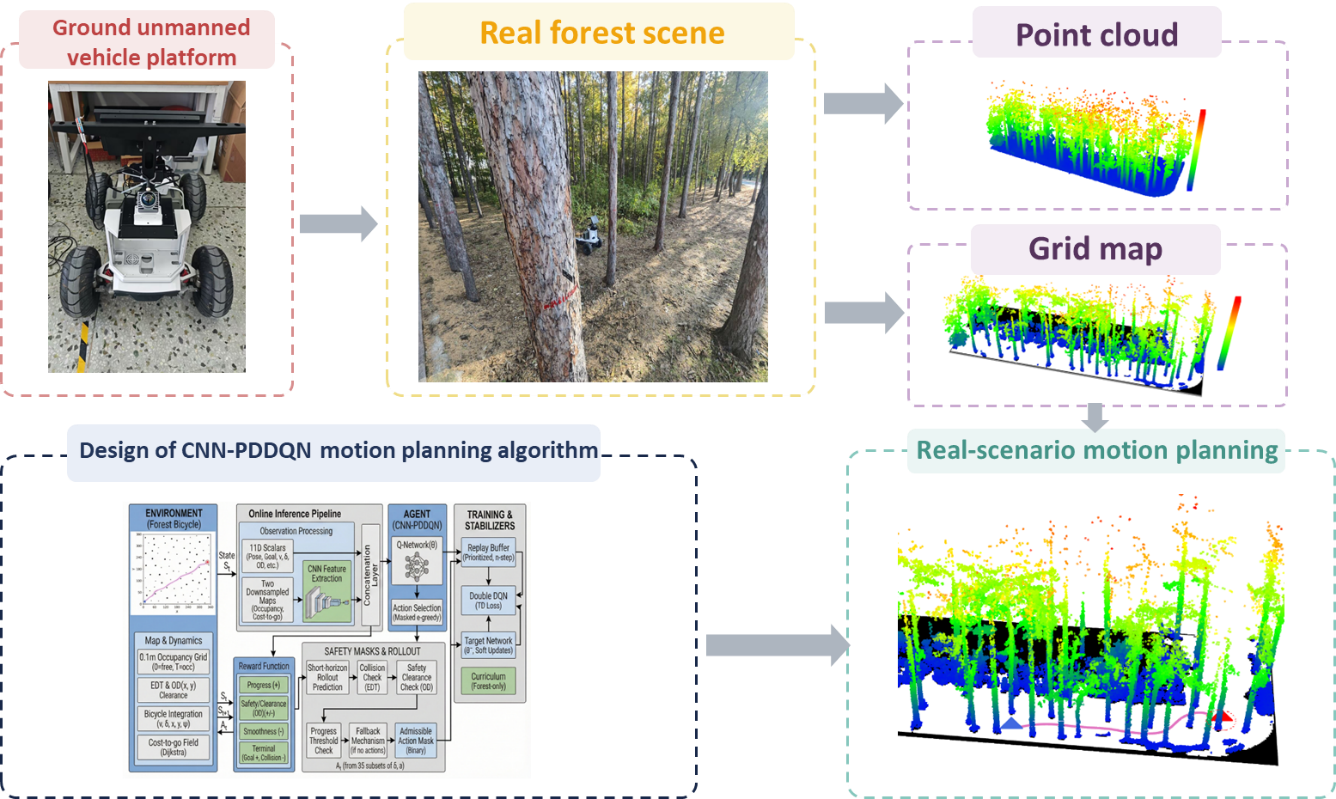
\includegraphics[width=\columnwidth]{fig_framework.png}
\caption{面向森林场景的UGV运动规划框架}
\label{fig:framework}
\end{figure}

\subsection{无人车与传感器}

实验平台采用阿克曼转向的地面无人车（UGV），如图~\ref{fig:platform}所示。硬件架构主要由运动底盘、感知套件与计算单元组成。运动方面，底盘采用前轮转向、后轮驱动的阿克曼结构，配备大尺寸充气轮胎与优良减震性能的悬架系统，以适应林间起伏路面。感知方面，传感器为Livox~Mid-360三维激光雷达，内置IMU并以30°俯角安装，能提供360°视场角与最远100\,m的测距能力。计算单元搭载Jetson AGX Orin 64g，运行Ubuntu系统和ROS，搭载SLAM建图与路径规划算法，并通过CAN通讯控制底盘。

\begin{figure}[t]
\centering
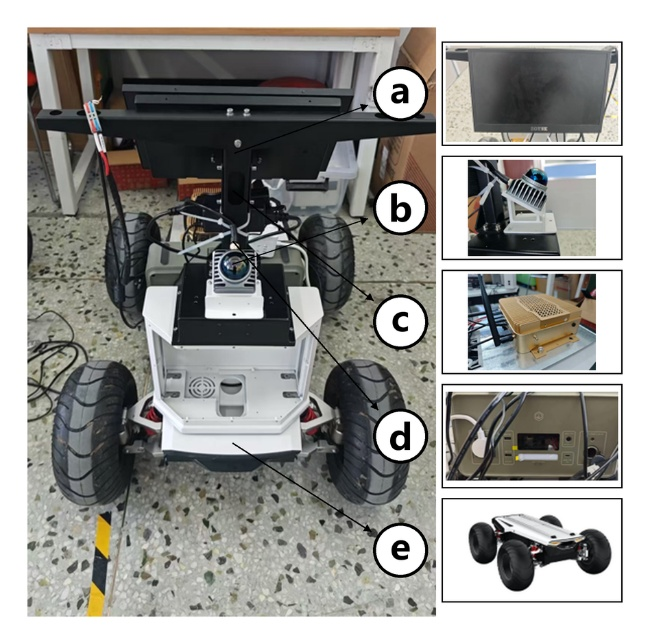
\includegraphics[width=0.65\columnwidth]{fig_platform.jpg}
\caption{地面无人车实验平台}
\label{fig:platform}
\end{figure}

\subsection{基于FAST-LIO2的先验点云地图的建立}

为建立三维点云地图，本文采用FAST-LIO2算法~\cite{xu2022fastlio2}，通过融合激光雷达与IMU数据，估计UGV在世界坐标系下的位姿与轨迹。将第$k$帧点云表示为集合$\mathcal{P}_{k} = \{p_{k,i}\}_{i=1}^{N_k}$，其中$p_{k,i} = [x_{k,i},y_{k,i},z_{k,i}]^\mathsf{T}$定义于激光雷达坐标系。FAST-LIO2输出该帧在全局坐标系下的位姿$T_k = [R_k, t_k]$，点云变换关系为：
\begin{equation}
  p_{k,i}^{g} = R_k\, p_{k,i} + t_k
\end{equation}
其中$p_{k,i}^{g}$为全局坐标系下的点坐标。所有变换后的点集增量式地融合至全局地图中。建图后对生成的点云地图进行降采样与统计离群点移除滤波（SOR）。

\subsection{基于可通行评估的点云分割}

给定全局坐标系下的点云地图$\mathcal{M} = \{\mathbf{p}_i\}_{i=1}^{N}$。对每个点$\mathbf{p}_i$定义半径为$r$的邻域$\mathcal{N}_r(\mathbf{p}_i)$，计算局部坡度角：
\begin{equation}
  \theta_{ij} = \arctan\!\left(\frac{|z_i - z_j|}{\sqrt{(x_i-x_j)^2+(y_i-y_j)^2}}\right)
\end{equation}
设地面无人车的最大爬坡角为$\alpha_{\max}$，引入松弛因子$\lambda \in [0,1]$，统计邻域内超过坡度阈值的点数比例$r_{\text{slope}}$：
\begin{equation}
  r_{\text{slope}} = \frac{1}{|\mathcal{N}(p_i)|}\sum_{p_j\in\mathcal{N}(p_i)}\mathbb{I}(\alpha_{ij} > \alpha_{\max})
\end{equation}
若$r_{\text{slope}} \leq \lambda$，则认为点$p_i$所在的局部地形可通行；否则标记为不可通行点。

\subsection{地面无人车路径规划}

\subsubsection{车辆参数与运动学建模}

在全局坐标系下采用等效自行车模型描述车辆运动状态，如图~\ref{fig:kinematics}所示。选取车辆后轴中心为参考点，车辆状态定义为$s=(x,y,\theta)$，控制输入为$u=(v,\delta)$，其中$L$为轴距，$v$为线速度，$\delta$为前轮转角。在低速规划场景中，运动学方程为：
\begin{align}
  \dot{x} &= v\cos\theta, \quad
  \dot{y} = v\sin\theta, \quad
  \dot{\theta} = \frac{v}{L}\tan\delta
\end{align}

\begin{figure}[t]
\centering
\subfloat[]{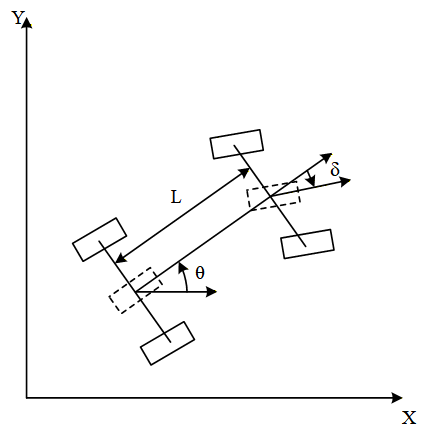
\includegraphics[width=0.48\columnwidth]{fig_kinematics_a.png}}
\hfill
\subfloat[]{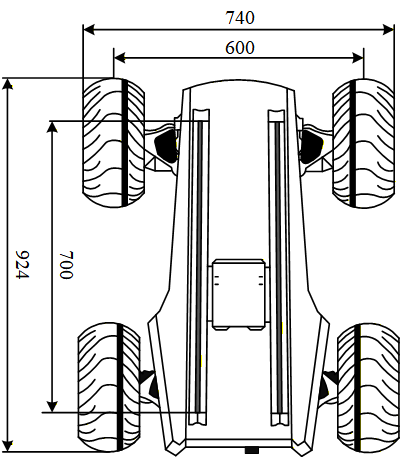
\includegraphics[width=0.48\columnwidth]{fig_kinematics_b.png}}
\caption{地面无人车运动学模型}
\label{fig:kinematics}
\end{figure}

\subsubsection{碰撞检测与代价场构建}

如图~\ref{fig:dual_circle}所示，采用``双圆足迹''对车体进行近似：以两个半径为$r$的圆分别覆盖车体前、后关键区域，圆心沿车体纵向分别位于参考点前后偏移$x_1$与$x_2$处。

\begin{figure}[t]
\centering
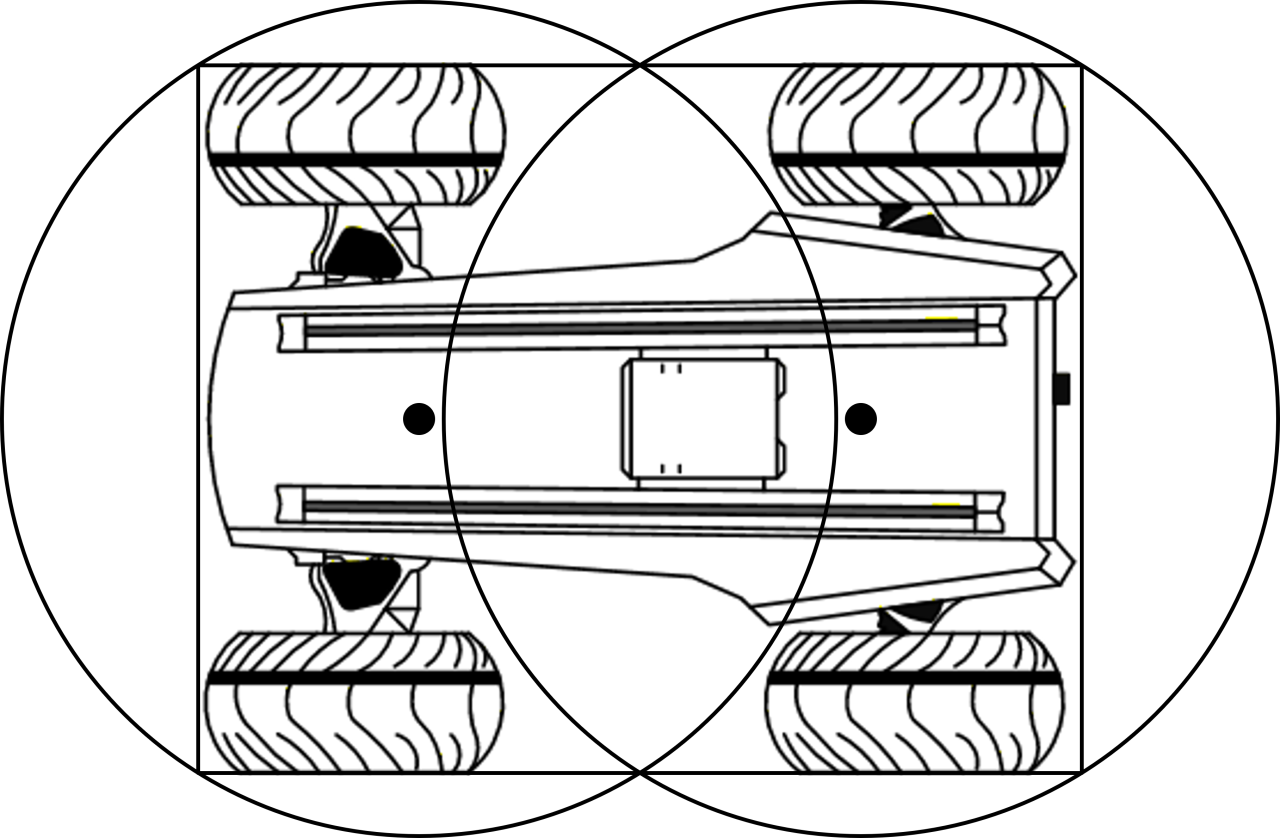
\includegraphics[width=0.55\columnwidth]{fig_dual_circle.png}
\caption{车辆双圆足迹示意图}
\label{fig:dual_circle}
\end{figure}

对于车辆姿态$(x,y,\theta)$，两圆心在全局坐标系中的位置为：
\begin{align}
  c_1 &= \bigl(x + \cos\theta\cdot x_1,\; y + \sin\theta\cdot x_1\bigr) \\
  c_2 &= \bigl(x + \cos\theta\cdot x_2,\; y + \sin\theta\cdot x_2\bigr)
\end{align}
若任一圆与障碍栅格发生重叠，则判定为碰撞。在构建到目标的代价场时，分别查询两圆心对应的到目标代价并取最大值：
\begin{equation}
  C_{\text{pose}}(x,y,\theta) = \max\bigl(C(c_1),\, C(c_2)\bigr)
\end{equation}

\subsubsection{马尔可夫决策过程（MDP）建模}

MDP表示为四元组$M=(S,A,P,R)$。

\textbf{状态空间}$S$：三维环境的特征信息被映射到二维网格中，每个栅格地图的分辨率为$0.1$\,m。状态的前11维为低维标量状态（归一化后的智能体/目标位置、航向正余弦、速度与转角的归一化量等），其余部分为两张大小为$N\times N$的全局栅格图。

\textbf{动作空间}$A$：构造动作查找表$\mathbf{T}\in\mathbb{R}^{35\times2}$，每个动作对应一组$[\dot{\delta}, a]$：
\begin{equation}
  A = \{(\dot{\delta}_i, a_j) \mid \dot{\delta}_i\in\Delta_{\dot{\delta}},\, a_j\in\Delta_a\},\quad |A|=7\times5=35
\end{equation}
其中$\dot{\delta}_{\max}=60°/\text{s}$，$a_{\max}=1.5$\,m/s$^2$，$dt=0.05$\,s，$v_{\max}=2.0$\,m/s，$\delta_{\max}=27°$。

\textbf{奖励函数}：总奖励为：
\begin{equation}
  R_t = r_{\text{prog}} + r_{\text{time}} + r_{\text{smooth}} + r_{\text{safety}} + r_{\text{term}}
\end{equation}

\textit{A.~进度奖励}：令$C(s)$为考虑绕障的代价场，则进度奖励$r_{\text{prog}} = k_p(C(s_t) - C(s_{t+1}))$。

\textit{B.~时间惩罚}：$r_{\text{time}} = -k_t$，鼓励更快完成规划。

\textit{C.~平滑与可控性约束}：引入控制平滑项与曲率惩罚：$r_{\delta} = -k_{\delta}(\delta_{t+1}-\delta_t)^2$，$r_a = -k_a(a_t-a_{t-1})^2(v_{t+1}/v_{\max})^2$，$r_{\kappa} = -k_{\kappa}\tan^2(\delta_{t+1})$。

\textit{D.~安全无碰撞奖励}：取两圆心到最近障碍边界距离$d_1,d_2$，圆半径为$r$，则$OD(s)=\min(d_1-r,\,d_2-r)$。若$OD<d_s$，采用反距离差构造惩罚：
\begin{equation}
  r_{\text{obs}} = -\min\!\left(k_{\text{obs,max}},\, k_o\!\left(\frac{1}{OD+\varepsilon}-\frac{1}{d_s+\varepsilon}\right)\right)
\end{equation}

\subsubsection{基于CNN-PDDQN的深度强化学习路径规划策略}

在MDP建模基础上，采用CNN对局部占据栅格/代价图进行特征提取，并以CNN-PDDQN学习离散动作的价值函数，如图~\ref{fig:cnn_pddqn}所示。

\begin{figure}[t]
\centering
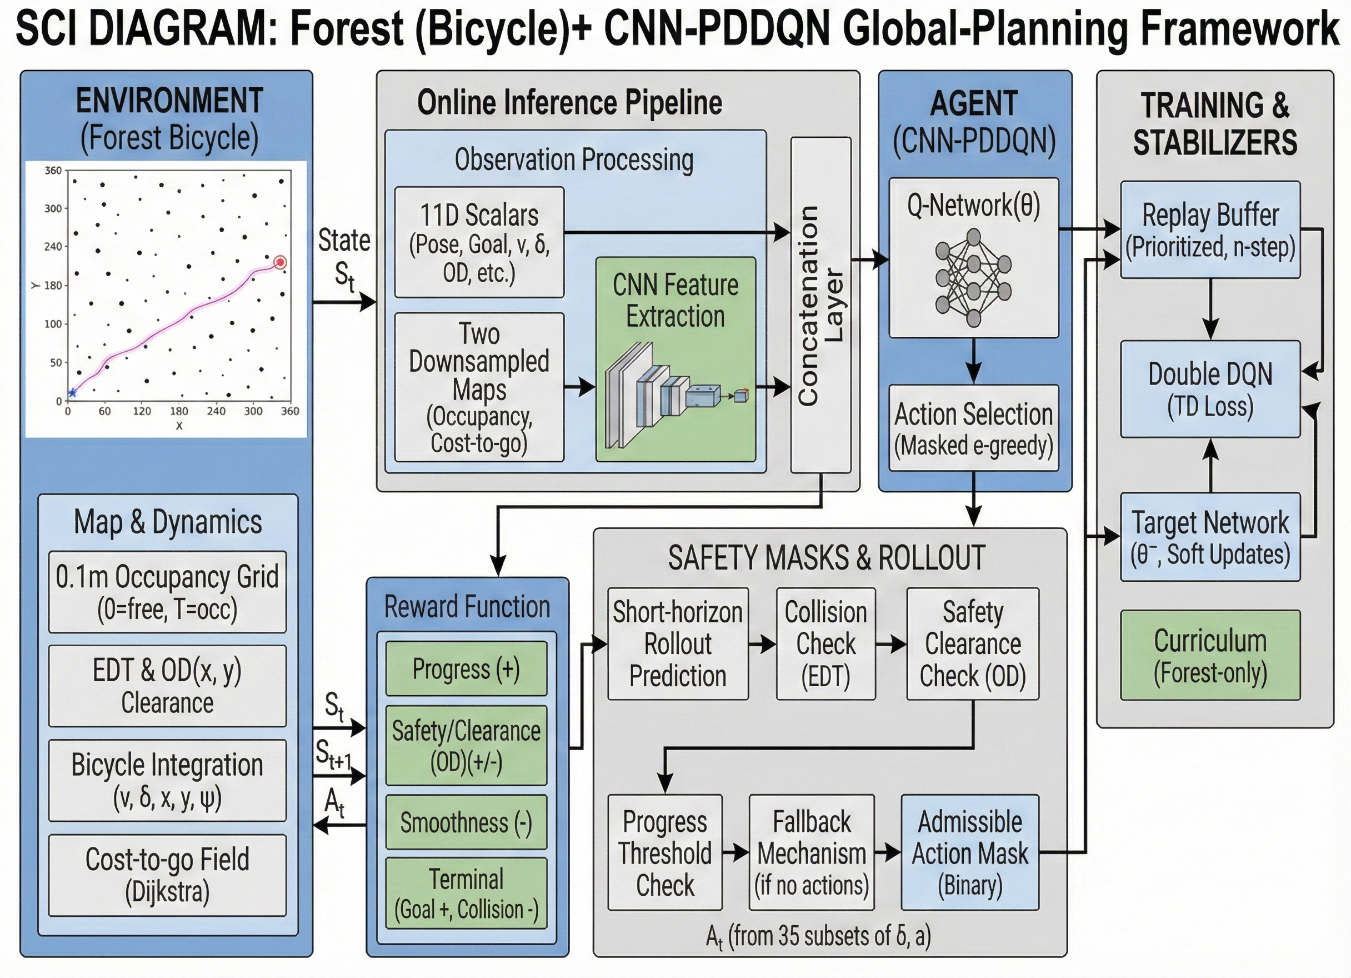
\includegraphics[width=\columnwidth]{fig_cnn_pddqn.png}
\caption{CNN-PDDQN路径规划策略的在线推理与训练框架}
\label{fig:cnn_pddqn}
\end{figure}

\textbf{CNN-Q网络结构}：CNN编码器由3层2D卷积与ReLU组成（无池化层，以步长实现下采样），参数如表~\ref{tab:cnn_structure}所示。

\begin{table}[t]
\centering
\caption{CNN编码器结构参数}
\label{tab:cnn_structure}
\footnotesize
\begin{tabular}{@{}ccccc@{}}
\toprule
\textbf{层} & \textbf{卷积核} & \textbf{stride} & \textbf{padding} & \textbf{输出通道} \\
\midrule
Conv1 & $3\times3$ & 1 & 1 & 32 \\
Conv2 & $3\times3$ & 2 & 1 & 64 \\
Conv3 & $3\times3$ & 2 & 1 & 64 \\
\bottomrule
\end{tabular}
\end{table}

最终Q函数以拼接特征为输入输出35维动作价值向量：$\mathbf{Q}(s,\cdot) = f_\theta(\mathbf{h})\in\mathbb{R}^{35}$，输入维度为$11+d_{\text{cnn}}$，输出维度为35。

\textbf{自适应动作选择策略}：为降低选择``高Q但不可执行动作''的概率，引入在线可行域过滤机制。对任一候选动作$a_i$，在固定预测步长$H$内保持控制量不变，进行前向积分得到预测轨迹$\hat{x}_{t+1:t+H}^{(i)}$，据此定义可采纳动作集合：
\begin{equation}
  A_{\text{adm}}(s_t) = \{a_i\in A \mid c_i=0,\, d_i^{\min}\geq d_{\text{thr}},\, (\Delta J_i\geq\eta)\vee\text{reached}\}
\end{equation}

掩码化$\varepsilon$-greedy贪心选择：
\begin{equation}
  a_t = \arg\max_{a_i\in A}\bigl(Q_\theta(s_t,a_i) + (1-m_i)\cdot(-\infty)\bigr)
\end{equation}

\textbf{目标网络}采用Polyak平均（软更新）进行平滑跟踪：
\begin{equation}
  \bar{\theta} \leftarrow (1-\tau)\bar{\theta} + \tau\theta
\end{equation}

对于样本$(s,a,R^{(n)},s',\text{done},n)$，Double~DQN的$n$-step~TD目标写为：
\begin{equation}
  y = \begin{cases} R^{(n)}, & \text{done}=1 \\ R^{(n)}+\gamma^n Q_{\bar{\theta}}(s',a^*), & \text{otherwise} \end{cases}
\end{equation}
其中$a^* = \arg\max_{a'\in A(s')}Q_\theta(s',a')$，并最小化Huber损失更新$\theta$。

完整训练与在线规划伪代码如图~\ref{fig:algorithm}所示。

\begin{figure}[t]
\centering
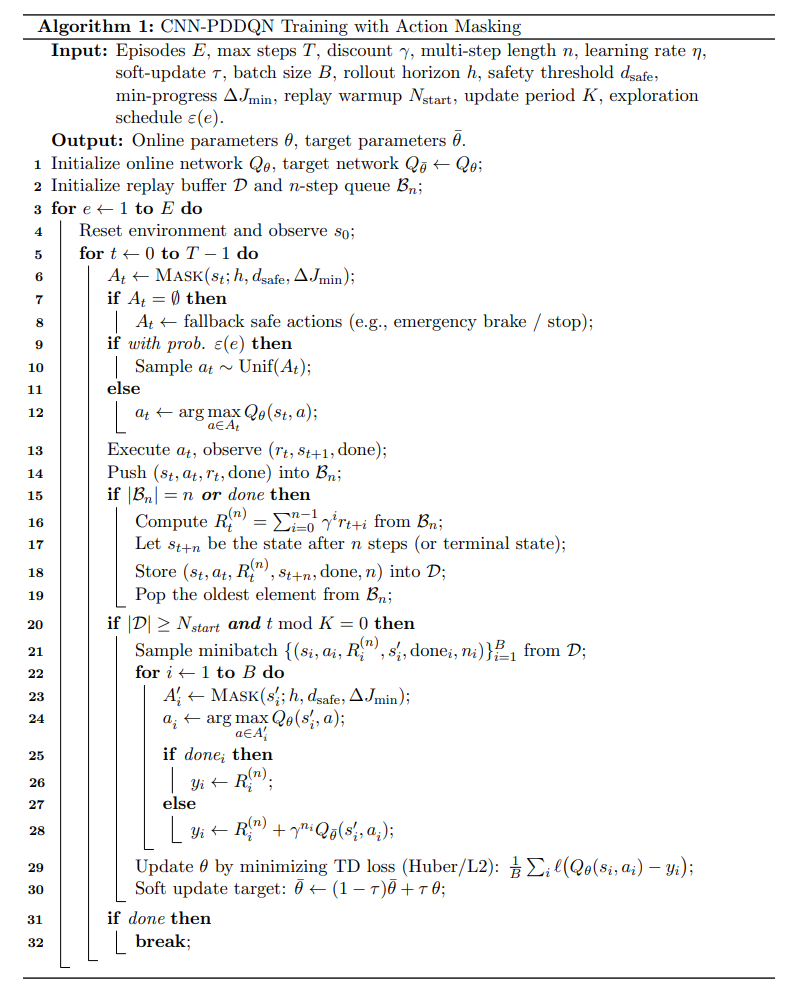
\includegraphics[width=0.88\columnwidth]{fig_algorithm.png}
\caption{CNN-PDDQN训练与在线规划流程（伪代码）}
\label{fig:algorithm}
\end{figure}

% ══════════════════════════════════════════════════════════════
\section{结果与讨论}\label{sec:results}

为系统评估方法的可行性与有效性，在PyCharm平台实现了所提算法及对比算法的统一仿真框架，并构建仿真森林环境开展对比测试。

\subsection{基准算法}

本文选取Hybrid A*、SS-RRT*以及DQN系列强化学习算法（MLP/CNN两种网络结构）进行对比。

\subsection{评价指标}

设置四项评价指标：路径长度$L$（m）、平均绝对曲率$\bar{\kappa}$（m$^{-1}$）、规划耗时$T$（s）以及综合得分$S$。对任一指标$x\in\{L,\bar{\kappa},T\}$，其归一化形式为：
\begin{equation}
  \tilde{x} = \frac{x - x_{\min}}{x_{\max} - x_{\min} + \varepsilon}
\end{equation}
综合得分$S = 1 - \frac{\tilde{L}+\tilde{\bar{\kappa}}+\tilde{T}}{3}$，越大越好。

\subsection{仿真场景下的对比验证}

\subsubsection{长路径对比}

将训练完成的模型部署到随机森林仿真场景中进行测试，随机生成10组起点与终点，图~\ref{fig:sim_long}展示了其中两次规划结果。

\begin{figure}[t]
\centering
\subfloat[]{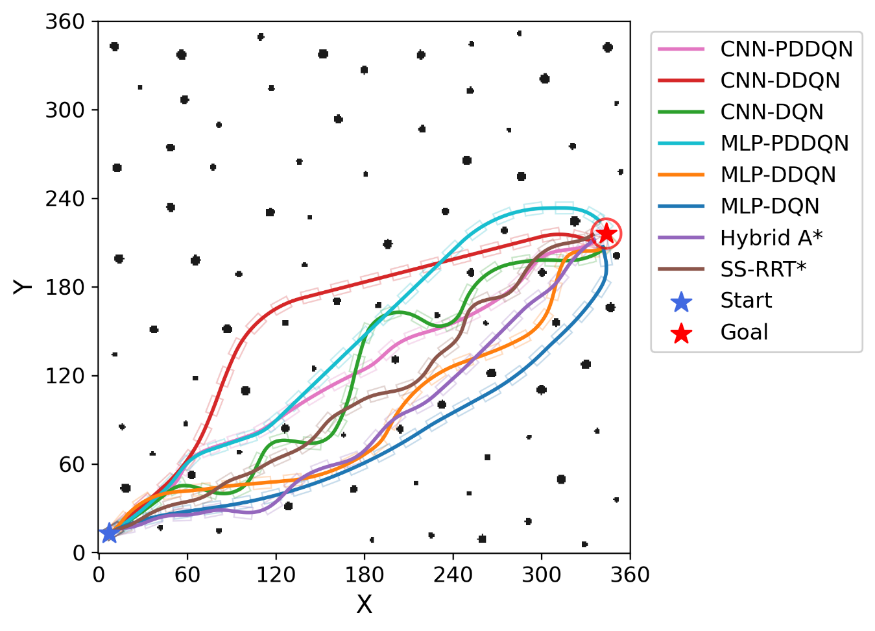
\includegraphics[width=0.48\columnwidth]{fig_sim_long_a.png}}
\hfill
\subfloat[]{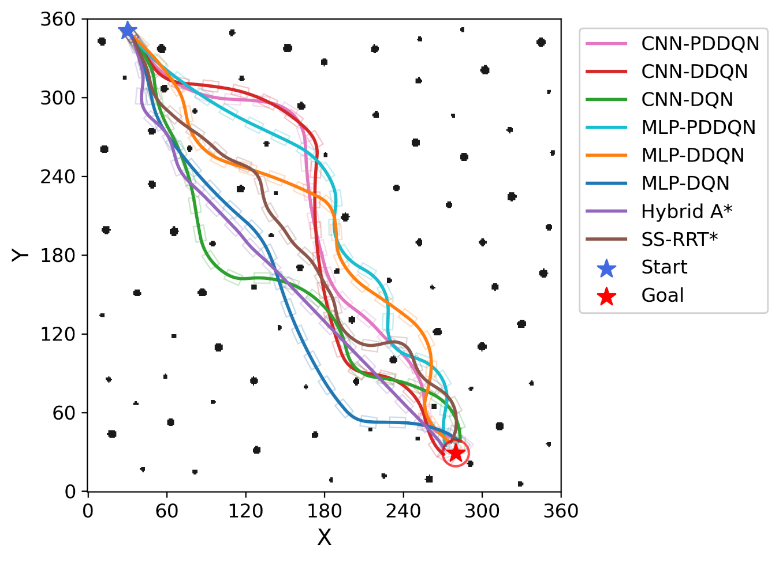
\includegraphics[width=0.48\columnwidth]{fig_sim_long_b.png}}
\caption{随机森林仿真场景下长路径任务的规划结果对比示例}
\label{fig:sim_long}
\end{figure}

\begin{table}[t]
\centering
\caption{长路径任务中不同算法的平均性能指标对比}
\label{tab:long_path}
\footnotesize
\begin{tabular}{@{}lccccc@{}}
\toprule
\textbf{算法} & \textbf{成功率} & \textbf{路径(m)} & \textbf{曲率(1/m)} & \textbf{耗时(s)} & \textbf{得分} \\
\midrule
CNN-PDDQN  & 1.0 & \textbf{40.197} & \textbf{0.097} & 0.269 & \textbf{0.078} \\
CNN-DDQN   & 1.0 & 40.815 & 0.117 & 0.288 & 0.174 \\
CNN-DQN    & 1.0 & 41.216 & 0.108 & 0.273 & 0.183 \\
MLP-PDDQN  & 1.0 & 40.866 & 0.104 & \textbf{0.191} & 0.170 \\
MLP-DDQN   & 1.0 & 44.136 & 0.166 & 0.205 & 0.482 \\
MLP-DQN    & 1.0 & 44.136 & 0.166 & 0.173 & 0.479 \\
Hybrid A*  & 1.0 & 40.651 & 0.104 & 3.569 & 0.357 \\
RRT*       & 0.9 & 41.537 & 0.262 & 1.608 & 0.596 \\
\bottomrule
\end{tabular}
\end{table}

\begin{figure}[t]
\centering
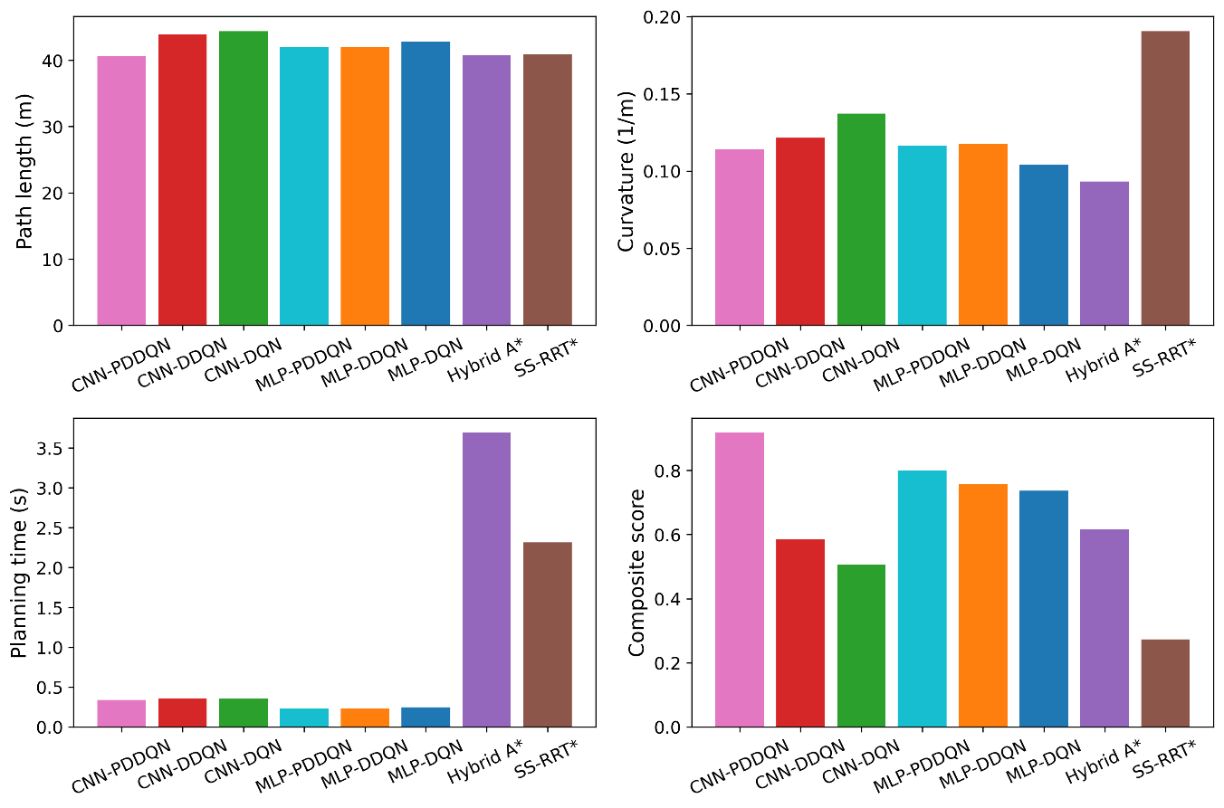
\includegraphics[width=\columnwidth]{fig_bar_long.png}
\caption{长路径任务中不同算法的平均性能指标对比柱状图}
\label{fig:bar_long}
\end{figure}

表~\ref{tab:long_path}展示了各算法在长路径任务上的平均指标。所有6种DQN变体的成功率均达到100\%（RRT*为90\%），表明深度强化学习方法在长距离规划中具有良好的可靠性。在路径质量方面，CNN-PDDQN生成了最短路径（40.197\,m）与最低平均曲率（0.097\,m$^{-1}$），优于Hybrid\,A*（40.651\,m、0.104\,m$^{-1}$）。在规划效率方面，所有DQN变体的规划耗时均低于0.3\,s，而Hybrid\,A*为3.569\,s、RRT*为1.608\,s，DQN方法的实时性优势显著。

\subsubsection{短路径对比}

进一步构造起终点距离更近的短路径任务，图~\ref{fig:sim_short}给出了两组典型结果，表~\ref{tab:short_path}和图~\ref{fig:bar_short}汇总了各算法在短路径任务上的平均指标。

\begin{figure}[t]
\centering
\subfloat[]{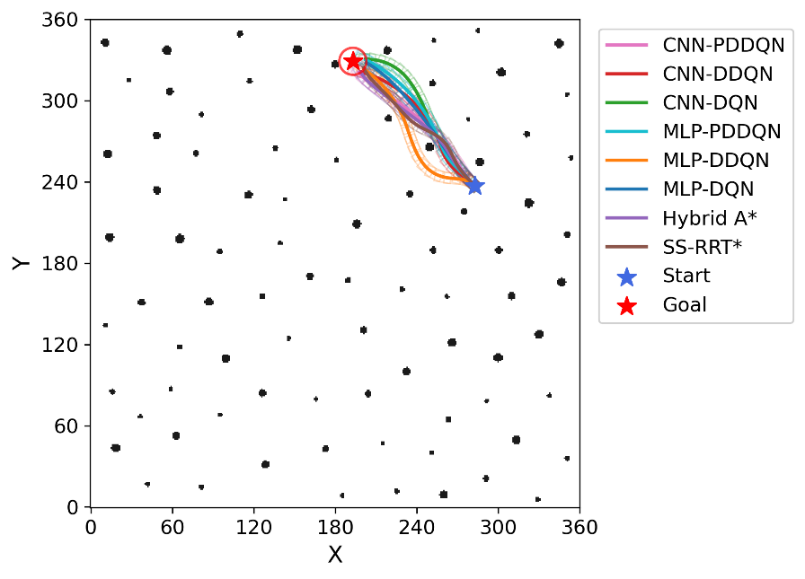
\includegraphics[width=0.48\columnwidth]{fig_sim_short_a.png}}
\hfill
\subfloat[]{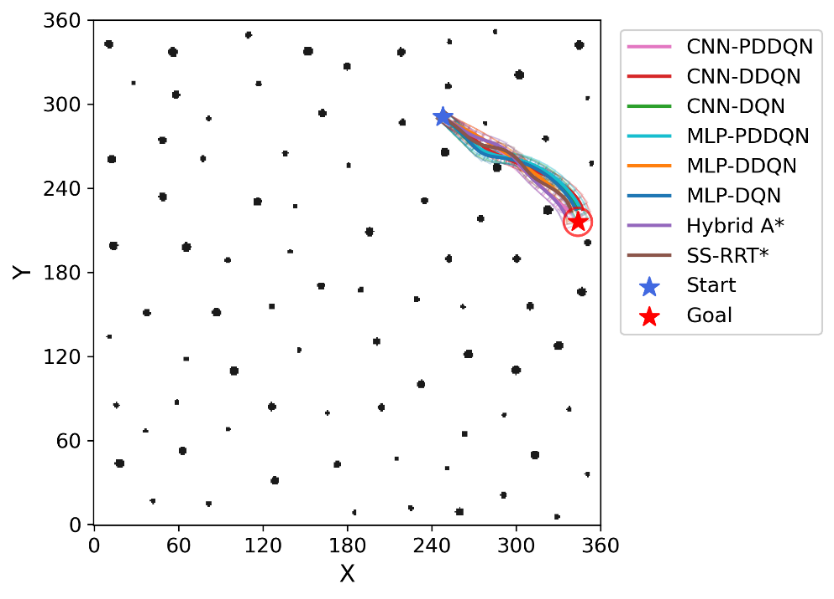
\includegraphics[width=0.48\columnwidth]{fig_sim_short_b.png}}
\caption{随机森林仿真场景下短路径任务的规划结果对比示例}
\label{fig:sim_short}
\end{figure}

\begin{table}[t]
\centering
\caption{短路径任务中不同算法的平均性能指标对比}
\label{tab:short_path}
\footnotesize
\begin{tabular}{@{}lccccc@{}}
\toprule
\textbf{算法} & \textbf{成功率} & \textbf{路径(m)} & \textbf{曲率(1/m)} & \textbf{耗时(s)} & \textbf{得分} \\
\midrule
CNN-PDDQN  & 0.9 & 8.954 & 0.166 & 0.086 & 0.260 \\
CNN-DDQN   & 0.9 & 9.043 & 0.150 & 0.094 & 0.241 \\
CNN-DQN    & 0.9 & 8.961 & \textbf{0.109} & 0.110 & \textbf{0.164} \\
MLP-PDDQN  & \textbf{1.0} & \textbf{8.966} & 0.169 & \textbf{0.055} & 0.267 \\
MLP-DDQN   & 0.9 & 9.519 & 0.117 & 0.081 & 0.262 \\
MLP-DQN    & 0.9 & 9.519 & 0.117 & 0.101 & 0.267 \\
Hybrid A*  & \textbf{1.0} & 8.993 & 0.113 & 1.752 & 0.340 \\
RRT*       & \textbf{1.0} & 9.449 & 0.292 & 0.078 & 0.383 \\
\bottomrule
\end{tabular}
\end{table}

\begin{figure}[t]
\centering
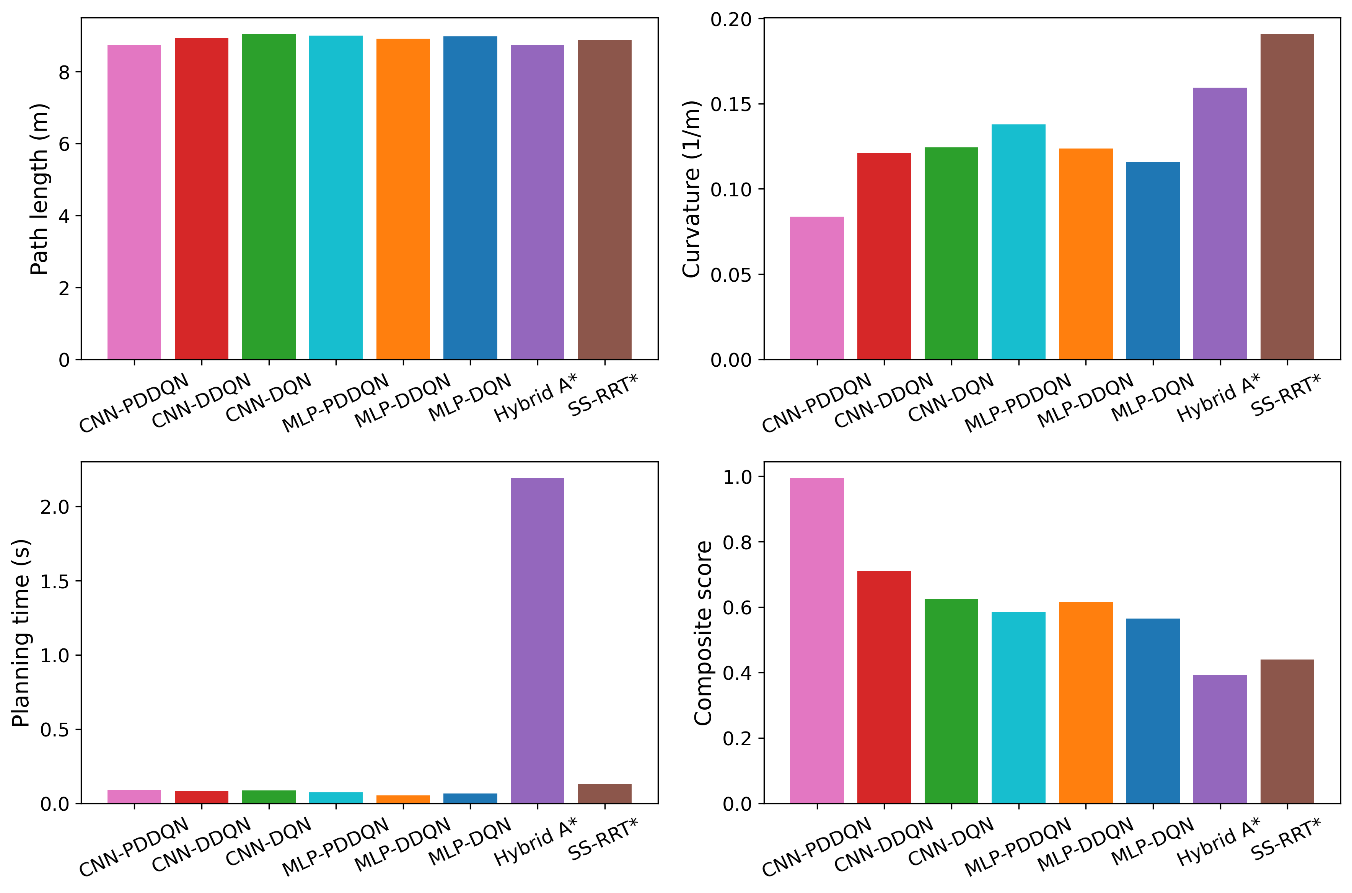
\includegraphics[width=\columnwidth]{fig_bar_short.png}
\caption{短路径任务中不同算法的平均性能指标对比柱状图}
\label{fig:bar_short}
\end{figure}

从表~\ref{tab:short_path}可见，在短路径任务中，MLP-PDDQN的成功率最高（100\%），规划耗时仅0.055\,s。CNN-DQN的平均曲率最低（0.109\,m$^{-1}$），路径最为平滑。所有DQN变体的规划耗时均低于0.11\,s，远优于Hybrid\,A*（1.752\,s）。传统方法Hybrid\,A*虽然成功率保持100\%，但规划耗时高出一个数量级；RRT*成功率100\%但曲率较大（0.292\,m$^{-1}$），路径平滑性不足。

\subsection{真实场景下的对比验证}

\subsubsection{真实场景的建立}

为验证所提方法在真实林地环境中的可行性与泛化能力，在中国黑龙江省哈尔滨市东北林业大学森林试验场建立真实场景的先验点云地图，如图~\ref{fig:realmap_site}所示。

\begin{figure}[t]
\centering
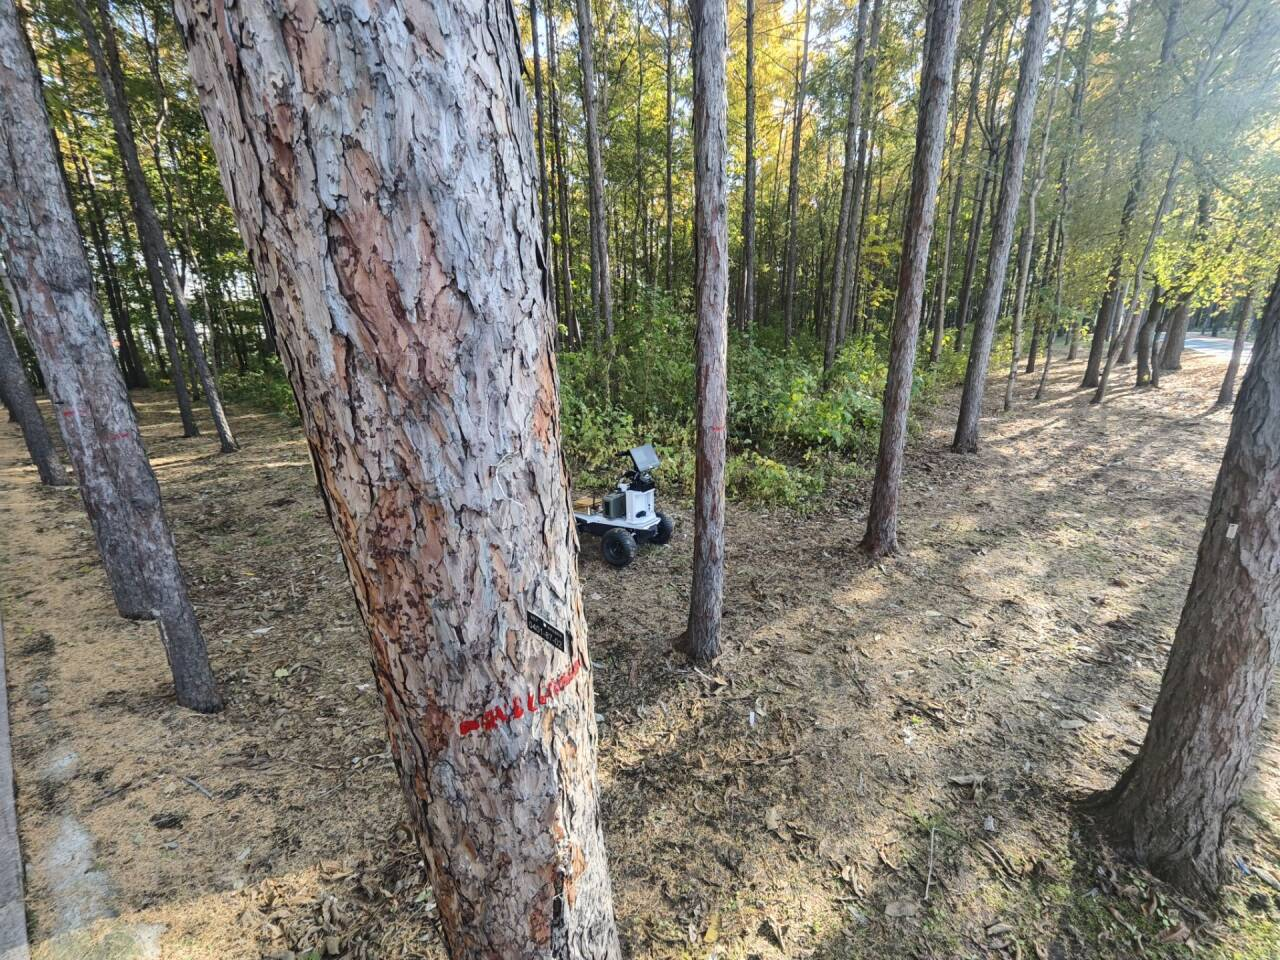
\includegraphics[width=0.6\columnwidth]{fig_realmap_site.png}
\caption{真实林地试验场景}
\label{fig:realmap_site}
\end{figure}

按照第~\ref{sec:method}节所述流程，采用FAST-LIO2构建三维点云先验地图，并对地图进行体素降采样与统计离群点移除（SOR）滤波，结果如图~\ref{fig:pointcloud}所示。

\begin{figure}[t]
\centering
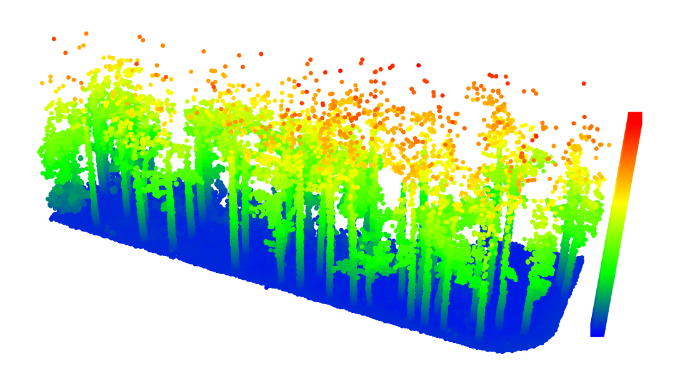
\includegraphics[width=0.85\columnwidth]{fig_pointcloud.png}
\caption{FAST-LIO2构建后降采样与SOR滤波后的三维点云先验地图}
\label{fig:pointcloud}
\end{figure}

在点云先验地图基础上，采用第~\ref{sec:method}节提出的可通行性评估对点云进行分割，并将分割结果投影生成二维占据栅格地图，如图~\ref{fig:traversability}所示。

\begin{figure}[t]
\centering
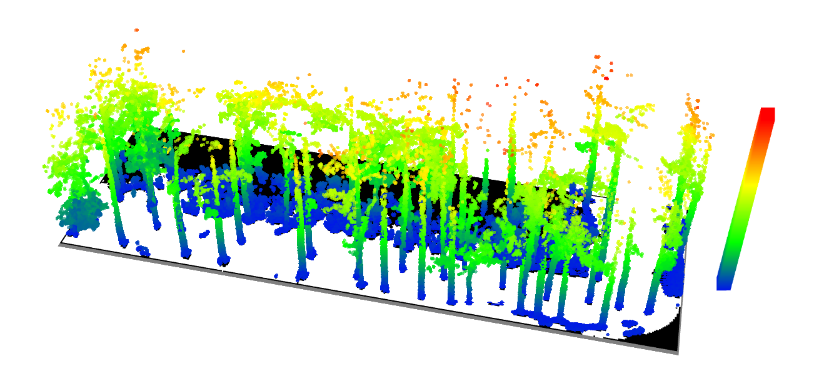
\includegraphics[width=0.85\columnwidth]{fig_traversability.png}
\caption{可通行性分割结果及带点云的栅格地图}
\label{fig:traversability}
\end{figure}

\subsubsection{真实场景下的结果}

在上述地图与车辆运动学约束条件下，将CNN-PDDQN与多种基线算法在相同起终点条件下进行对比测试。图~\ref{fig:real_paths}给出了代表性轨迹结果，表~\ref{tab:real_short}与表~\ref{tab:real_long}分别汇总了短路径与长路径任务中各算法的平均性能指标。

\begin{figure*}[t]
\centering
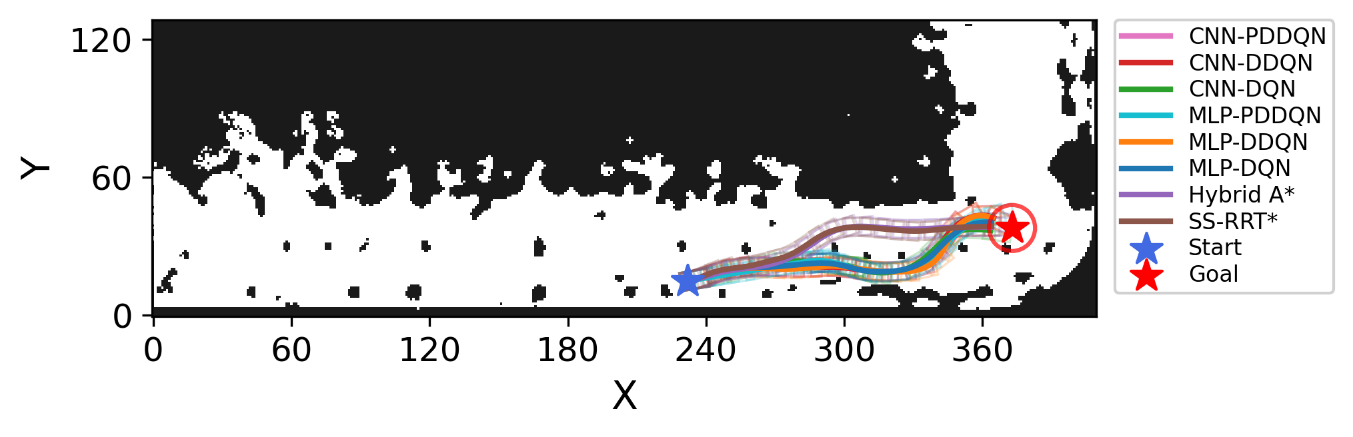
\includegraphics[width=\textwidth]{fig_real_paths.png}
\caption{真实林地场景下路径规划算法对比}
\label{fig:real_paths}
\end{figure*}

\begin{table}[t]
\centering
\caption{真实林地短路径任务中不同算法的平均性能指标对比}
\label{tab:real_short}
\footnotesize
\begin{tabular}{@{}lccccc@{}}
\toprule
\textbf{算法} & \textbf{成功率} & \textbf{路径(m)} & \textbf{曲率(1/m)} & \textbf{耗时(s)} & \textbf{得分} \\
\midrule
CNN-PDDQN  & 0.75 & \textbf{7.606} & 0.203 & 0.170 & 0.371 \\
CNN-DDQN   & 0.85 & 7.921 & 0.220 & 0.110 & 0.410 \\
CNN-DQN    & 0.75 & 7.992 & 0.216 & 0.199 & 0.414 \\
MLP-PDDQN  & 0.90 & 8.136 & 0.185 & \textbf{0.069} & 0.307 \\
MLP-DDQN   & 0.90 & 8.217 & 0.195 & 0.076 & 0.306 \\
MLP-DQN    & 0.85 & 8.030 & 0.237 & 0.086 & 0.408 \\
Hybrid A*  & \textbf{1.00} & 7.858 & \textbf{0.202} & 1.510 & 0.400 \\
RRT*       & 0.95 & 8.368 & 0.308 & 0.408 & 0.492 \\
\bottomrule
\end{tabular}
\end{table}

\begin{table}[t]
\centering
\caption{真实林地长路径任务中不同算法的平均性能指标对比}
\label{tab:real_long}
\footnotesize
\begin{tabular}{@{}lccccc@{}}
\toprule
\textbf{算法} & \textbf{成功率} & \textbf{路径(m)} & \textbf{曲率(1/m)} & \textbf{耗时(s)} & \textbf{得分} \\
\midrule
CNN-PDDQN  & 0.70 & 22.611 & 0.145 & 0.218 & 0.536 \\
CNN-DDQN   & 0.80 & 21.942 & 0.128 & 0.277 & 0.419 \\
CNN-DQN    & 0.95 & 22.738 & 0.152 & 0.205 & 0.414 \\
MLP-PDDQN  & 0.75 & 23.020 & 0.143 & 0.196 & 0.548 \\
MLP-DDQN   & \textbf{0.95} & \textbf{21.907} & \textbf{0.110} & \textbf{0.134} & \textbf{0.216} \\
MLP-DQN    & 0.85 & 22.391 & 0.129 & 0.155 & 0.335 \\
Hybrid A*  & \textbf{1.00} & 22.010 & 0.080 & 2.541 & 0.366 \\
RRT*       & 0.80 & 21.667 & 0.321 & 2.084 & 0.754 \\
\bottomrule
\end{tabular}
\end{table}

\begin{figure}[t]
\centering
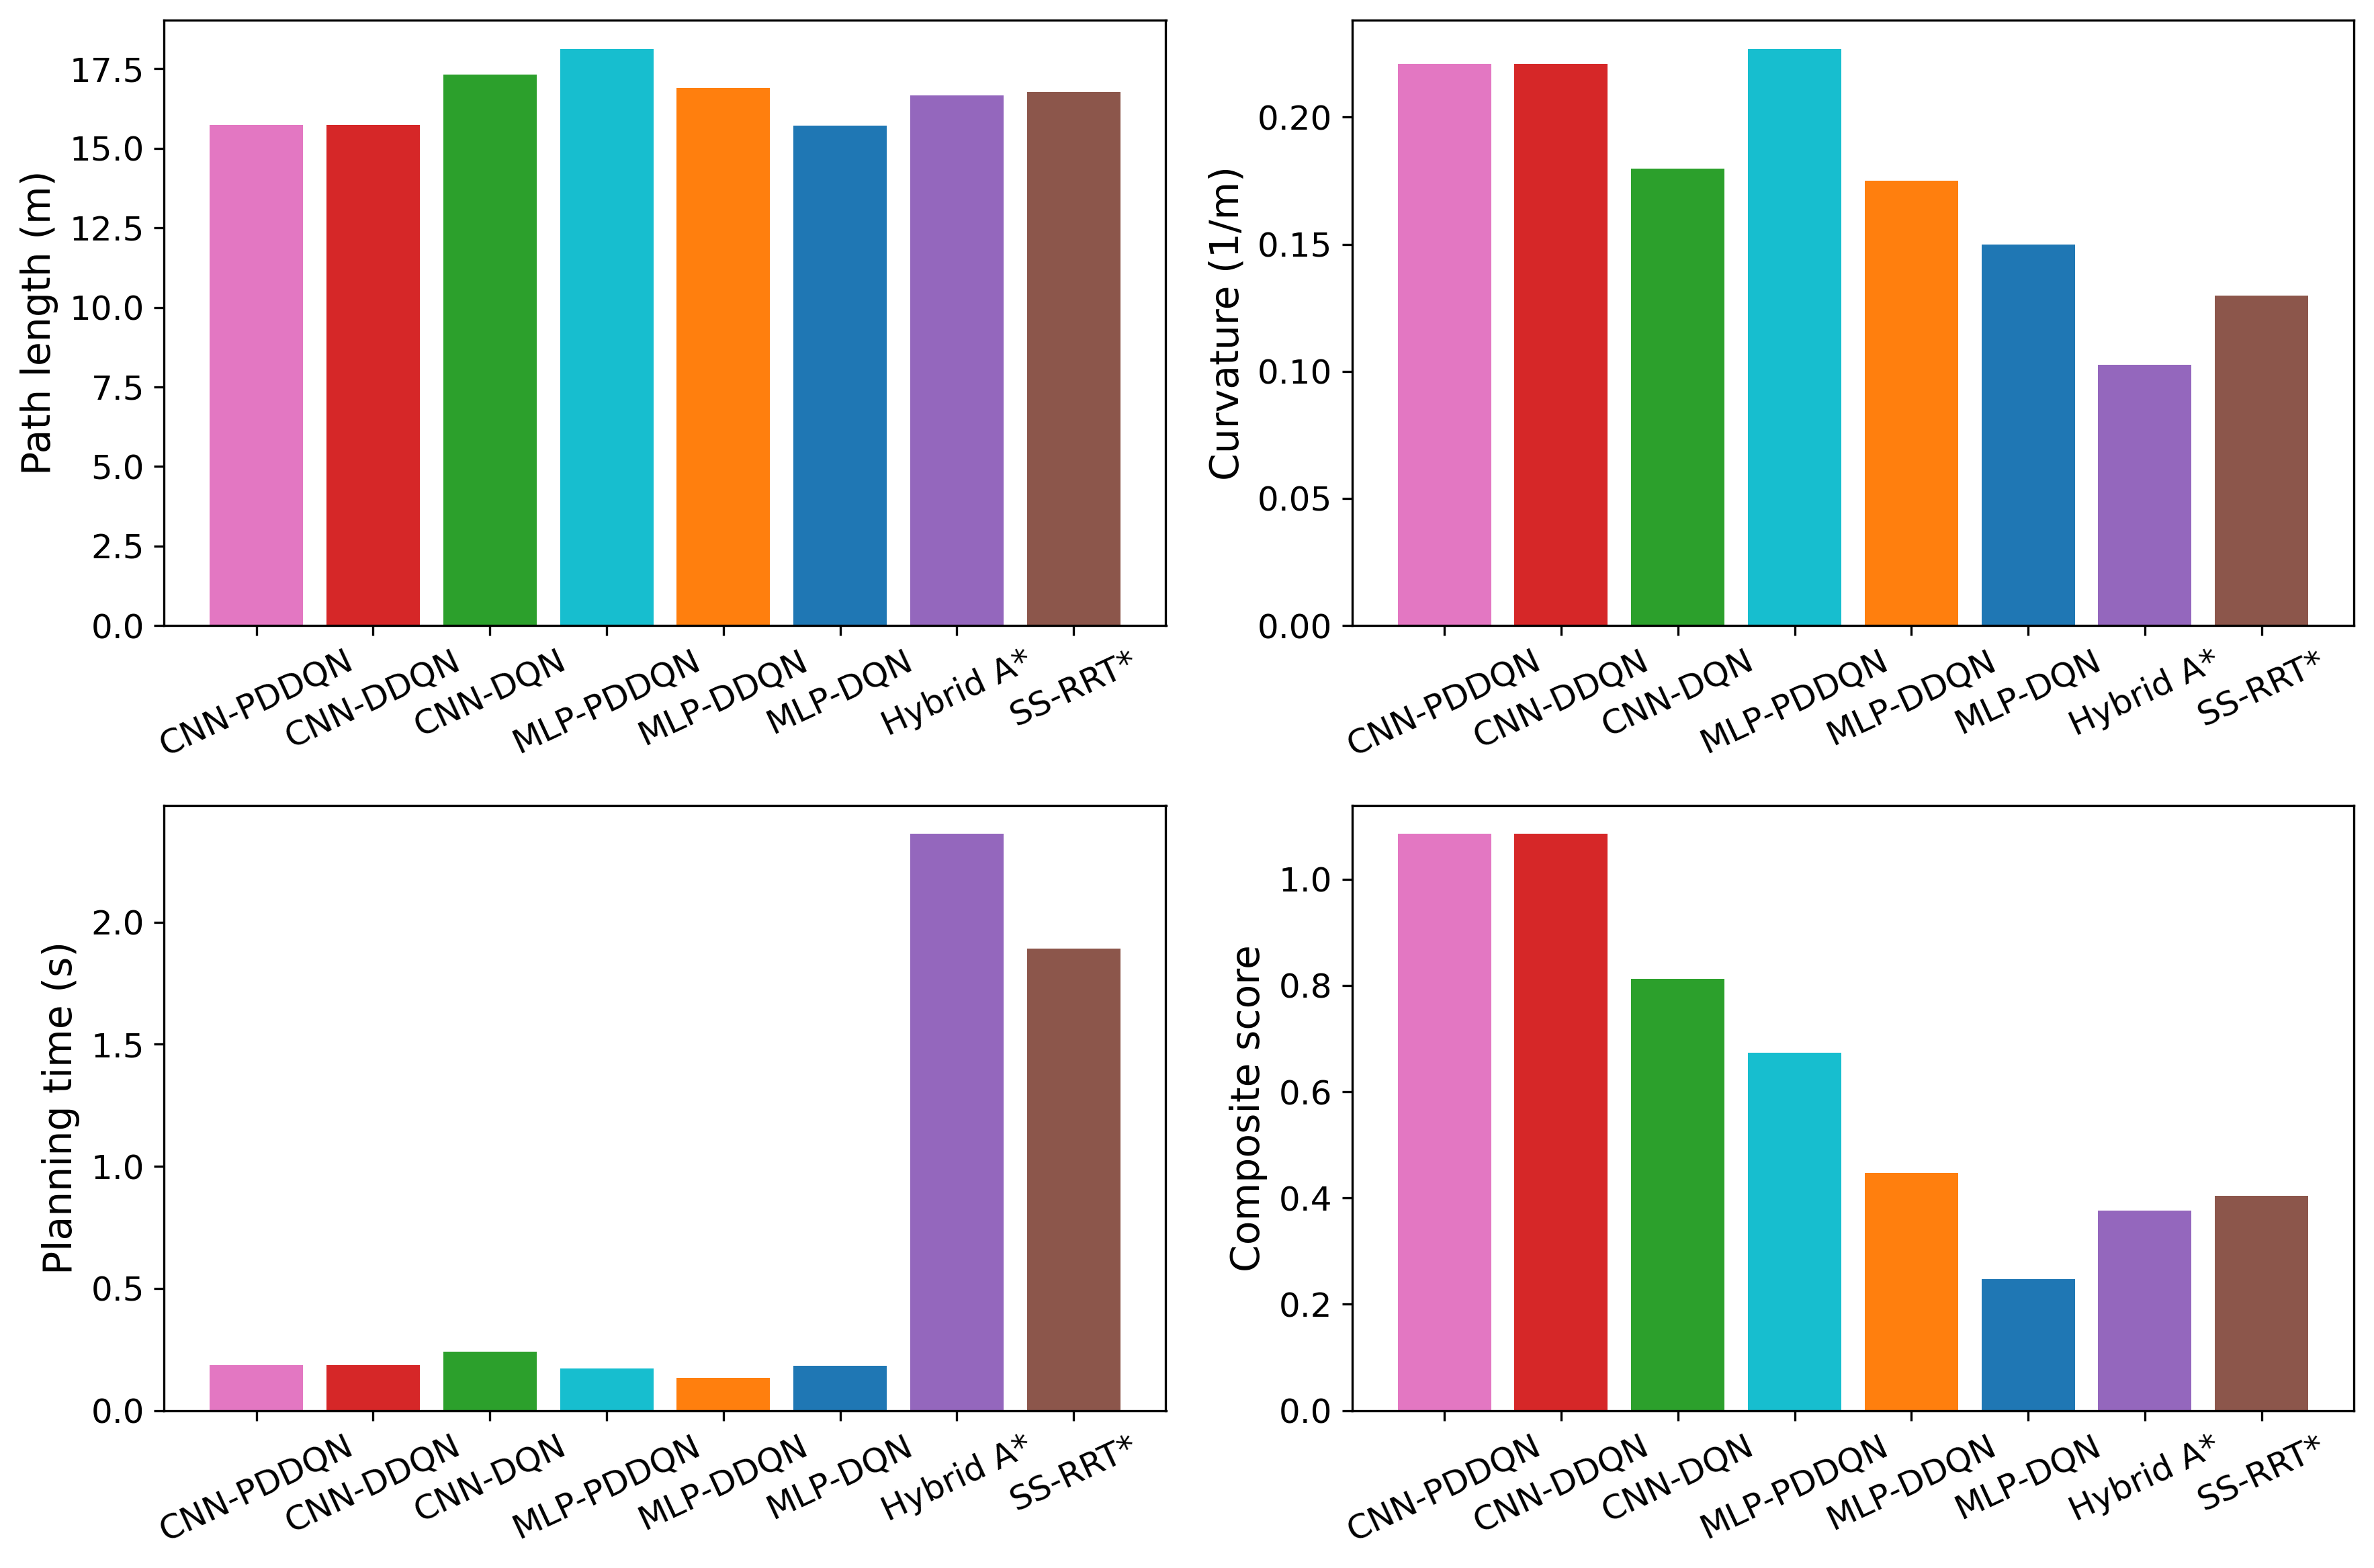
\includegraphics[width=\columnwidth]{fig_bar_real.png}
\caption{真实林地实验中不同算法的平均性能指标对比柱状图}
\label{fig:bar_real}
\end{figure}

从表~\ref{tab:real_short}和表~\ref{tab:real_long}可见，在真实林地短路径任务中，MLP-PDDQN和MLP-DDQN均取得90\%的最高DRL成功率，MLP-PDDQN规划耗时仅0.069\,s。在长路径任务中，MLP-DDQN取得95\%的成功率与最短路径（21.907\,m），规划耗时仅0.134\,s。相比之下，Hybrid\,A*虽然成功率为100\%，但规划耗时高达2.541\,s。整体来看，DQN变体的规划耗时比传统方法低约一个数量级，具有显著实时性优势。CNN-PDDQN在真实地图中成功率偏低（短路径75\%，长路径70\%），分析原因在于真实林地的走廊结构与森林仿真差异较大，PDDQN的Polyak目标更新在此类非均匀环境中收敛较慢。

\subsection{消融实验}\label{sec:ablation}

为进一步验证所提方法中各设计选项的有效性，设计了两组消融实验。

\subsubsection{奖励函数设计消融}

在forest\_a环境下分离分析goal proximity shaping与速度约束对成功率的影响，设置4个变体：A（无goal shaping，无速度约束）、B（加入接近奖励）、C（加入宽松速度约束$v_{\text{tol}}=1.0$\,m/s）和D（加入严格速度约束$v_{\text{tol}}=0.5$\,m/s），各训练300轮。表~\ref{tab:ablation_reward}汇总了RL算法的平均成功率。

\begin{table}[t]
\centering
\caption{奖励函数消融实验（6种RL算法平均成功率）}
\label{tab:ablation_reward}
\footnotesize
\begin{tabular}{@{}lcccc@{}}
\toprule
\textbf{场景} & \textbf{A（基线）} & \textbf{B（+shaping）} & \textbf{C（+speed 1.0）} & \textbf{D（+speed 0.5）} \\
\midrule
Short & \textbf{0.92} & 0.88 & 0.72 & 0.67 \\
Long  & \textbf{0.95} & 0.87 & 0.43 & 0.33 \\
\bottomrule
\end{tabular}
\end{table}

结果表明：（1）goal proximity shaping（A→B）对整体成功率略有负面影响，个别算法（MLP-DQN）提升明显但CNN-PDDQN退化严重；（2）速度约束带来的负面效应更为显著，C变体在长路径场景的RL平均成功率从0.87暴跌至0.43，D变体进一步降至0.33，表明300轮训练不足以令RL学会精确减速停车；（3）最终采用变体A（无shaping、无速度约束）的奖励设计。

\subsubsection{DQN+MPC两阶段架构消融}

测试``DQN全局规划+MPC局部跟踪''的两阶段架构相对纯DQN直接控制的性能差异。训练设置完全相同，仅推理管道不同：DQN先完成一次规划生成路标点，再由MPC沿路标执行跟踪。表~\ref{tab:ablation_mpc}对比了成功率变化。

\begin{table}[t]
\centering
\caption{DQN+MPC消融实验（RL均值成功率）}
\label{tab:ablation_mpc}
\footnotesize
\begin{tabular}{@{}lcc@{}}
\toprule
\textbf{场景} & \textbf{纯DQN} & \textbf{DQN+MPC} \\
\midrule
Short & \textbf{0.92} & 0.77 \\
Long  & \textbf{0.95} & 0.87 \\
\bottomrule
\end{tabular}
\end{table}

结果显示DQN+MPC整体不如纯DQN：Short成功率从0.92降至0.77（-16\%），Long从0.95降至0.87（-8\%）。根本原因在于，DQN生成的路径不保证可行性（可能绕路、陷入死角或未到达目标），MPC只能``盲目跟踪''，无法修正结构性路径缺陷。相比之下，传统方法（Hybrid A*）的两阶段架构成功率保持不变，因为其规划器保证生成完整可行路径。该结果验证了纯DQN直接控制的优越性。

% ══════════════════════════════════════════════════════════════
\section{结论}\label{sec:conclusion}

在树干密集、通道狭窄且地形起伏的森林非结构化环境中，为阿克曼式地面无人车（UGV）实现满足运动学约束的实时、安全、可执行路径规划，是提升森林巡检与作业自主化水平的关键。为此，本文提出一种面向森林场景的深度强化学习运动规划方法，融合先验三维建图、可通行性评估与约束感知策略学习，以实现实时、稳定且可执行的在线规划。

本研究的主要贡献如下：

\begin{enumerate}
  \item 构建了基于FAST-LIO2的先验点云建图与可通行性评估流程，实现点云分割并生成栅格地图。
  \item 将规划过程建模为马尔可夫决策过程，设计CNN-PDDQN价值网络，并结合进度、时间、平滑/可控性与双圆足迹安全裕度构造奖励函数，生成更短、更稳的可执行路径。
  \item 提出推理阶段的约束感知机制，引入在线动作掩码与短视滚动预测的可行域过滤，并配合回退机制与分层验证，减少必碰撞/低收益动作选择与振荡风险。
  \item 在随机森林仿真与真实林地场景中进行了充分对比验证：仿真长路径任务中CNN-PDDQN生成最短路径（40.197\,m）且规划耗时仅0.269\,s；真实林地长路径中MLP-DDQN成功率达95\%、规划耗时仅0.134\,s，均显著低于传统方法。消融实验进一步验证了奖励函数设计与纯DQN直接控制策略的有效性。
\end{enumerate}

\ack{[TODO: 致谢相关人员、机构和资金支持（可注明课题编号和资助方）]}

\section*{利益冲突声明}

作者声明不存在可能影响本文所报告工作的已知竞争性财务利益或个人关系。

% ══════════════════════════════════════════════════════════════
\bibliographystyle{unsrt}
\bibliography{references}

\end{document}
